\documentclass[border=5pt]{standalone}

\usepackage{amsfonts,amssymb,amsmath}
\usepackage{tikz}
\usetikzlibrary{matrix}

\newcommand{\zz}{\ensuremath\mathbb{Z}_2}
\newcommand{\Z}{\ensuremath\mathbb{Z}}

\tikzset{ 
table/.style={
  matrix of nodes,
  row sep=-\pgflinewidth,
  column sep=-\pgflinewidth,
  nodes={rectangle,text width=3em,align=center},
  text depth=1.25ex,
  text height=2.5ex,
  nodes in empty cells
},
row 1/.style={nodes={fill=gray!20,text depth=0.4ex,text height=2ex}},
column 1/.style={nodes={rectangle, text width=4em,align=center}}
}

\begin{document}
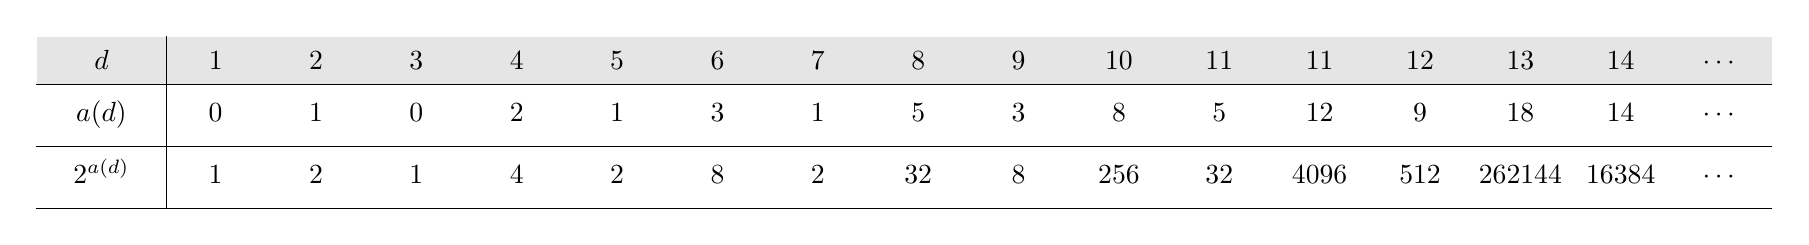
\begin{tikzpicture}
\matrix (mat) [table] {
    $d$ & $1$ & $2$ & $3$ & $4$ & $5$ & $6$ & $7$ & $8$ & $9$ & $10$ & $11$ &  $11$ & $12$ & $13$ & $14$ &  $\cdots$ \\
    $a(d)$ & $0$ & $1$ & $0$ & $2$ & $1$ & $3$ & $1$ & $5$ & $3$ & $8$ & $5$ & $12$ & $9$ & $18$ & $14$ & $\cdots$ \\
    $2^{a(d)}$ & $1$ & $2$ & $1$ & $4$ & $2$ & $8$ & $2$ & $32$ & $8$ & $256$ & $32$ & $4096$ & $512$ & $262144$ & $16384$ & $\cdots$ \\
};
% the matrix rules
\foreach \x in {1,...,3}
{
  \draw
    ([xshift=-.5\pgflinewidth]mat-\x-1.south west) --
    ([xshift=-.5\pgflinewidth]mat-\x-17.south east);
  }
\draw
    ([yshift=.5\pgflinewidth]mat-1-1.north east) --
    ([yshift=.5\pgflinewidth]mat-3-1.south east);
\end{tikzpicture}
\end{document}
